\chapter{Discrete Element Method - DEM}
\label{chap:DEM}
    Numerical simulations are widely used to study granular systems, which play an important role in complementing experimental information, which further enhances the understanding of granular physics phenomena. A justification to the use of numerical simulations is the precise control of the input parameters of the simulations and the level of complexity about the object of study. Another advantage is the extraction of data, that goes from the grain scale (microscale), such as positions and velocity of grains, rising to the scale of force chains (mesoscale), up to the system scale (macroscale), such as material shear, showing possible emerging properties and their causes.

    The technique to simulate of granular materials that we use in this work is a DEM known in the literature as Molecular Dynamics (MD). The method consists of numerically solving the Newton's laws of motion. An advantage of this method is that any force that can describe the interaction with the elements is accepted in this method.

    The technique described in the reference \cite{Computer_Simulation_of_Liquids} uses the formalisms of analytical mechanics through the interaction potentials between agents, whether Lagrangian or Hamiltonian potentials, to establish the forces acting on each agent. The disadvantage of this type of description is that dissipative forces may not appear, since the description of forces is directly related to potentials. Formally, the system must obey the set of Equations \label{equ:lagrange} described by the Lagrangian function of the system: 
\begin{subequations}
    \label{equ:lagrange}
    \begin{empheq}[left={}]{align}
        \label{equ:lagrange1}
        \mathcal{L} = \mathcal{T} - \mathcal{V},\\
        \label{equ:lagrange2}
        \sum_{k} \left[\frac{d}{dt} \left( \frac{\partial \mathcal{L}}{\partial \dot{q_k}} \right) - \left(\frac{\partial \mathcal{L}}{\partial q_k} \right)\right] = 0,\\
        \label{equ:lagrange_forca}
        \vec{F}_{i} = \nabla \mathcal{L} = -\nabla \mathcal{V},
    \end{empheq}
\end{subequations}
where $\mathcal{L}$ represents the Lagrangian function that governs the dynamics of the system, $\mathcal{T}$ the kinetic energy, $\mathcal{V}$ the potential energy, $k$ the number of generalized coordinates of the system, $q_{k}$ the generalized coordinates, $\dot{q_{k}}$ the generalized velocities, $\vec{F}_{i}$ the force exerted on the particle $i$ originated by the gradient of the potential $\mathcal{V}$. The disadvantage of this formulation is that only conservative forces are expressed due to the Lagrangian formulation. To solve this issue, we use the force description instead of the potential and kinetic energy.

    Other references \cite{Abraao-Dissertacao, Caio-Tese, Srdjan-Tese, Felipe-Tese, Nathalia-Dissertacao, Leticia-Dissertacao, Fabiola-Dissertacao, Dissertacao, Luding-Tese, Caio-Dissertacao, Bouzid-Tese, Wassgren-Tese, Computational_Granular_Dynamics} use the model directly from the acting forces about each element.

\section{Equations of motion}
    To carry out the simulation, the set of Equations \ref{equ:movimento} must be satisfied, which takes into account Newton's laws of motion. Thus, there is information on the agents' states as a function of time. 
\begin{subequations}
    \label{equ:movimento}
    \begin{empheq}[left={Translational}\empheqlbrace]{align}
        \label{equ:posicao_linear}
        \vec{r}_{i}(t) &= \vec{r}_{i}(0) + \int_{0}^{t} \vec{v}_{i}(t) dt,\\
        \label{equ:velocidade_linear}
        \vec{v}_{i}(t) &= \vec{v}_{i}(0) + \int_{0}^{t} \vec{a}_{i}(t) dt,\\
        \label{equ:aceleracao_linear}
        \vec{a}_{i}(t) &= \sum_{j} \frac{\vec{F}_{i,j}(t)}{m_{i}},
    \end{empheq}
    \begin{empheq}[left={Rotational}\empheqlbrace]{align}
        \label{equ:posicao_angular}
        \theta^{k}_{i}(t) &= \theta^{k}_{i}(0) + \int_{0}^{t} \vec{\omega}^{k}_{i}(t) dt,\\
        \label{equ:velocidade_angular}
        \vec{\omega}^{k}_{i}(t) &= \vec{\omega}^{k}_{i}(0) + \int_{0}^{t} \vec{\alpha}^{\;k}_{i}(t) dt,\\
        \label{equ:aceleracao_angular}
        \vec{\alpha}^{\;k}_{i}(t) &= {I^{k}_{i}}^{-1} \sum_{j} \vec{\tau}^{\;k}_{i,j}(t),
    \end{empheq}
\end{subequations}
where $i$ is the i-th particle of the system, $\vec{r}_{i}(t)$ is the position vector of the center of mass of the body $i$ at the instant of time $t$, $\vec{v}_{i}(t)$ or $\vec{\dot{r}}_{i}(t)$ is the velocity of the center of mass of the body, $\vec{a}_{i}(t)$ or $\vec{\dot{v}}_{i}(t)$ or $\vec{\ddot{r}}_{i}(t)$ is the acceleration of the center of mass of the body, $\vec{F}_{i,j}(t)$ is the component of the force that the center of mass of the body suffers from interacting with another body or field $j$, $m_{i}$ is the body mass, $\theta^{k}_{i}(t)$ is angular position coordinates expressed in the system's $k$ basis, $\vec{\omega}^{k}_{i}(t)$ is the pseudovector of angular velocities of the body expressed on the basis $k$ of the system, $\vec{\alpha}^{k}_{i}(t)$ is the pseudovector of angular accelerations of the body, ${I^{k}_{i}}^{-1}$ is the inverse of the inertia tensor of the body and $\vec{\tau}^{k}_{i,j}(t)$ is the torque vector that the body suffers from interacting with another body or field. Remembering that the relationship between torque and the force that causes it can be described by the Equation \ref{equ:torque}:
\begin{equation}
    \label{equ:torque}
    \vec{\tau}_{i,j}(t) = \vec{\chi}_{i,j}(t) \times \vec{F}_{i,j}(t),
\end{equation}
where the vector $\vec{\tau}_{i,j}(t)$ is the torque on the particle $i$ caused by the contact forces with the body or field $j$. The vector $\vec{\chi}_{i,j}(t)$ is the vector that connects the center of mass of the particle $i$ to the point of application of the force, and the vector $\vec{F}_{i,j}(t)$ is the vector of the contact forces caused by interacting with another body or field $j$. The Equations \ref{equ:aceleracao_linear} and \ref{equ:aceleracao_angular} express Newton's second law. 

    The formulation described by the set of Equations \ref{equ:movimento} covers spaces in 1D, 2D and 3D, but this thesis focuses only on the formulation of 2D systems.

\subsection{Force model}
\label{subchap:Modelo_Forcas}
    The forces present in the systems modelled in this Chapter include the contact forces between agents and the gravitational force. The interaction forces between grain and fluid is described in Chapter \ref{chap:CFD}.

\subsubsection{Contact forces}
\label{subsubchap:Reologia}
    The contact forces model between grains we used to simulate granular materials was the rheological model proposed by Kelvin-Voigt \cite{Kelvin, Voigt}. Kelvin-Voigt rheology models the contact force between two grains by a spring and a damper in parallel in the normal direction of contact, as exemplified in Figure \ref{fig:forcas}. The normal spring represents the elastic contribution of the material, related to the Young's modulus, while the normal damper has the function of dissipate the energy in the inelastic collision between the grains. Additionally, a tangential spring is inserted in the tangential direction to play the role of the Coulomb friction. A model proposed in \cite{Caio-Tese} adds a damper-like element in parallel to the tangential spring, modelling the rolling resistance. We chose to use circular geometry for the grains. In consequence of the circular geometry, all angular momentum variation is caused by torque due to tangential force.

\begin{figure}[H]
    \begin{minipage}{.45\linewidth}
        \centering
        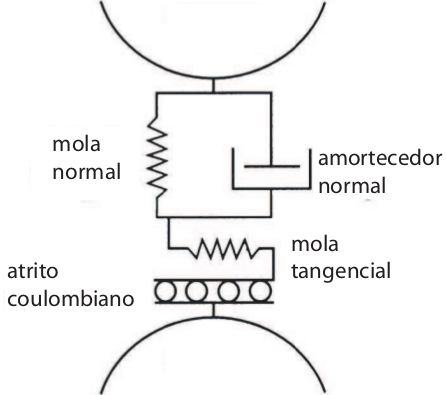
\includegraphics[width=0.9\textwidth]{04-figuras/Modelo_Forcas.png}
        \subcaption{Contact force model between agents. }
        \label{fig:forcas_modelo}
    \end{minipage}
    \begin{minipage}{.45\linewidth}
        \centering
        \includegraphics[width=0.9\textwidth]{04-figuras/Contato.tikz}
        \subcaption{Contact representation between grains.}
        \label{fig:forcas_contato}
    \end{minipage}
    \caption[Contact force model.]{Force model and representation between two circular grains. Figures taken from \cite{Sands_Powders_and_Grains}.}
    \label{fig:forcas}
\end{figure}

    A peculiarity of DEM is that it allows interpenetration between the grains. Therefore, in this model there is no deformation when two bodies are in contact. The maximum interpenetration we allow in our model is controlled by the material's hardness parameter and we impose a maximum penetration of $0.5\%$ of the radius.

    To determine the value of the interpenetration, $\delta$, in circular geometry, the Equation \ref{equ:interpenetracao}:
\begin{equation}
    \label{equ:interpenetracao}
    \delta_{i,j}^{\perp} = \left(R_{i}+R_{j}-\left|\vec{r}_{j}-\vec{r}_{i}\right|\right)\mathcal{H}(R_{i}+R_{j}-\left|\vec{r}_{j}-\vec{r}_{i}\right|),
\end{equation}
where $\delta_{i,j}^{\perp}$ is the value of the interpenetration between the grains $i$ and $j$, $R_{i}$ is the radius of the body $i$, $R_{j}$ is the radius of the body $j$, $\vec{r}_{i}$ is the position vector of the center of the body $i$, $\vec{r}_{j}$ is the position vector of the center of the body $j$ and $\mathcal{H}$ is the Heaviside step function. So, when the distance between the bodies is greater than the sum of the radii, the bodies will not be in contact and the Heaviside step function indicates that the interpenetration between the grains is null. If the distance between the bodies is lesser than the sum of the radii, the bodies will be in contact and the Heaviside step function indicates that there is interpenetration between grains, by its value being equals to one.

    With grains being in contact, the direct consequence of the interpenetration is the appearance of an elastic repulsive force, and the force depends on the interpenetration function $\delta^{\perp}$. The force expression can be calculated by the Equation \ref{equ:forca_elastica}: 
\begin{equation}
    \label{equ:forca_elastica}
    \vec{F}_{i,j}^{el} = -k_{n}\left(\delta_{i,j}^{\perp}\right)^{\frac{D}{2}}\hat{n}_{i,j},
\end{equation}
where $\vec{F}_{i,j}^{el}$ is the normal elastic force that the body $j$ causes to the body $i$ when they come in contact, $k_{n}$ is the constant related to the elasticity of the material in the direction of contact, $\delta_{i,j}^{\perp}$ is the interpenetration between the bodies $i$ and $j$, $D$ is the dimension of the system (in this case, $D=2$) and $\hat{n}_{i,j}$ is the normal direction of the contact \cite{Dissertacao, Caio-Tese, Landau}. One can write a potential for this elastic force as: $\mathcal{V} = \frac{1}{2}k_{n}\left({\delta_{i,j}^{\perp}}\right)^2$.

    Associated with the elastic force, the damping force is also present. As it is a dissipative force, a potential cannot be associated with the damping force. Most of the energy loss of granular materials is in collision. The Equation \ref{equ:forca_amortecimento} describes its behavior: 
\begin{equation}
    \label{equ:forca_amortecimento}
    \vec{F}_{i,j}^{am} = -\gamma \left(\vec{v}_{i,j}.\hat{n}_{i,j}\right)\hat{n}_{i,j},
\end{equation}
where $\vec{F}_{i,j}^{am}$ is the normal damping force that the body $j$ causes to the body $i$ when they come in contact, $\gamma$ is the damping constant related to the inelastic collision, $\vec{v}_{i,j}$ is the relative velocity between the centers of mass of bodies $i$ and $j$ and $\hat{n}_{i,j}$ is the normal contact direction \cite{Dissertacao, Caio-Tese, Computational_Granular_Dynamics}.

    The damping constant is directly linked to the restitution coefficient and can be used equivalently through the identities shown in the set of Equations \ref{equ:restituicao}. Some authors use the restitution coefficient in simulations, such as \cite{Srdjan-Tese, Luding-Tese, Computational_Granular_Dynamics}. In this thesis we will use the damping coefficient.

\begin{subequations}
    \begin{empheq}[left={}]{align}
        \epsilon &= \exp\left(\frac{-\pi}{\sqrt{\frac{4k_{n}m}{\gamma^2}-1}}\right),\\
        \gamma &= \sqrt{\frac{4k_{n}m}{\left(\frac{\pi}{\ln\left(\epsilon\right)}\right)^2+1}},
    \end{empheq}
    \label{equ:restituicao}
\end{subequations}
where $\epsilon$ is the restitution coefficient, $\gamma$ is the damping coefficient, $k_{n}$ is the stiffness related to the elasticity of the material and $m$ is the reduced mass $m=\frac{m_{i}m_{j}}{m_{i}+m_{j}}$.

    The friction force is also present in the simulation model. As the surfaces are in contact, there will be a frictional force between them if they tend to move each other. In particular, due to the circular geometry, friction forces will only act in the tangential direction. The relative velocity between the contact point of the bodies is given by the Equation \ref{equ:velocidade_relativa} below: 
\begin{equation}
    \label{equ:velocidade_relativa}
    \delta_{i,j}^{\parallel} = \vec{v}_{ij}.\hat{t}_{ij} - R_{i}\omega_{i} - R_{j}\omega_{j},
\end{equation}
where $\delta_{i,j}^{\parallel}$ is the relative velocity of the contact point of the bodies $i$ and $j$, $\vec{v}_{ij}$ is the relative velocity of the centers of mass of the bodies $i$ and $j$, $\hat{t}_{ij}$ is the tangential vector to the contact surfaces of the bodies $i$ and $j$, $R_{i}$ is the radius of the body $i$, $R_{j}$ is the radius of the body $j$, $\omega_{i}$ is the angular velocity of the body $i$ and $\omega_{j}$ is the angular velocity of the body $j$.

    For the tangential force, it is necessary to know the relative displacement of the contact point, as given by the equation \ref{equ:velocidade_relativa}, applied in the system of Equations \ref{equ:forca_atrito}, which models the Coulomb friction, and is given by:
\begin{equation}
    \label{equ:forca_atrito}
    \vec{F}_{i,j}^{at} = \left\{
    \begin{array}{l l l}
        \displaystyle -\int_{t_{0}}^{t_{f}} k_{t} \delta_{i,j}^{\parallel} \hat{t}_{ij}\, \mathrm{d} t, & \quad \textrm{if } k_{t} \left| \delta_{i,j}^{\parallel} \right| \leq \mu \left|\vec{F}_{i,j}^{n}\right| & \textrm{ (Static friction)} \\
        \displaystyle -\frac{\delta_{i,j}^{\parallel}}{\left|\delta_{i,j}^{\parallel}\right|} \mu \left| \vec{F}_{i,j}^{n} \right| \hat{t}_{ij}\, & \quad \textrm{if } k_{t} \left| \delta_{i,j}^{\parallel} \right| > \mu \left| \vec{F}_{i,j}^{n} \right| & \textrm{ (Kinetic friction)}
    \end{array}
    \right.\ ,
\end{equation}
where $\vec{F}_{i,j}^{at}$ is the friction force between the bodies $i$ and $j$, $k_{t}$ is the elastic constant of the material in the tangential direction, $\delta_{i,j}^{\parallel}$ is the relative velocity between the contact point of the bodies $i$ and $j$, $\hat{t}_{ij}$ is the tangential vector to contact surfaces of bodies $i$ and $j$, $\mu$ is the friction coefficient between the surfaces of bodies $i$ and $j$ and $\vec{F}_{i,j}^{n} = \vec{F}_{i,j}^{el} +\vec{F}_{i,j}^{am}$ is the force normal to the surfaces of bodies $i$ and $j$.

    We chose to model static and dynamic friction coefficient to be a single value for simplicity, presented the friction coefficient $\mu$. Figure \ref{fig:atrito} describe the Coulomb friction we use in the simulations.

\begin{figure}[H]
    \centering
    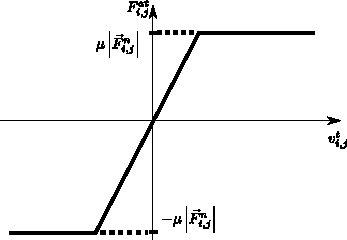
\includegraphics[width=0.5\textwidth]{04-figuras/Atrito.pdf}
    \caption[Friction.]{Friction versus relative velocity between contact. Figure taken from \cite{Caio-Tese}.}
    \label{fig:atrito}
\end{figure}

\subsubsection{The external force: Gravity}
\label{subsubchap:Gravidade}
    For this model, we assume that the gravitational force is a constant. For convenience, we normalize gravity as a unit value.

\subsubsection{The external force: The vibration}
    In the BNE problems, vibration must be present to agitate grains. One way to impose the vibration is to modulate an oscillatory force in the base where grains are. We chose to impose the variation in the position of walls instead of impose this variation in the force that sustains the walls.

\subsection{Temporal discretization}
    For the computational simulation of solid bodies, the kinematics equations must be rewritten as Taylor series expansions, and we chose the interpolating the velocity equation system by the algorithm known as Velocity Verlet \cite{Verlet, Computer_Simulation_of_Liquids}. The equations of motion discretized in time, as a function of the time step $\Delta t$, become as in the set of Equations \ref{equ:movimento_discreto}:
\begin{subequations}
    \label{equ:movimento_discreto}
    \begin{empheq}[left={Translational}\empheqlbrace]{align}
        \label{equ:posicao_linear_discreta}
        {\vec{r}_{i}}^{\;n+1} &= {\vec{r}_{i}}^{\;n} + {\vec{v}_{i}}^{\;n} \Delta t + \frac{{\vec{a}_{i}}^{\;n}}{2} (\Delta t)^{2},\\
        \label{equ:velocidade_linear_discreta}
        {\vec{v}_{i}}^{\;n+1} &= {\vec{v}_{i}}^{\;n} + \frac{{\vec{a}_{i}}^{\;n}+{\vec{a}_{i}}^{\;n+1}}{2} \Delta t,\\
        \label{equ:aceleracao_linear_discreta}
        {\vec{a}_{i}}^{\;n+1} &= \frac{\sum_{j} {\vec{F}_{i,j}}^{\;n+1} + \sum {\vec{F}_{i,ext}}^{\;n+1}}{m_{i}},
    \end{empheq}
    \begin{empheq}[left={Rotational}\empheqlbrace]{align}
        \label{equ:posicao_angular_discreta}
        {\theta_{i}}^{n+1} &= {\theta_{i}}^{n} + {\vec{\omega}_{i}}^{\;n} \Delta t + \frac{{\vec{\alpha}_{i}}^{\;n}}{2} (\Delta t)^{2},\\
        \label{equ:velocidade_angular_discreta}
        {\vec{\omega}_{i}}^{\;n+1} &= {\vec{\omega}_{i}}^{\;n} +\frac{{\vec{\alpha}_{i}}^{\;n}+{\vec{\alpha}_{i}}^{\;n+1}}{2} \Delta t,\\
        \label{equ:aceleracao_linear_discreta}
        {\vec{\alpha}_{i}}^{\;n+1} &= {I_{i}}^{-1} \sum_{j} {\vec{\tau}_{i,j}}^{\;n},
    \end{empheq}
\end{subequations}
where $i$ is the index of the moving body, $j$ is the index of the body in contact with the body $i$, $n$ is the time step, $\vec{r}$ is the position of the body, $\vec{v}$ is the velocity of the body, $\vec{a}$ is the acceleration of the body, $\Delta t$ is the size of the time step, $\vec{F}_{i,j}$ is the contact force between the bodies $i$ and $j$, $\vec{F}_{ext}$ are the external forces, such as gravity, $m$ is the mass of the body, $\theta$ is the angular position of the body, $\vec{\omega}$ is the angular velocity of the body, $\vec{\alpha}$ is the angular acceleration of the body, $\vec{\tau}$ is the torque on the body, $I$ is the moment of inertia of the body. 

    The set of Equations \ref{equ:movimento_discreto} is written for the 2D system, since there is only one degree of freedom for the rotation, and consequently all equations are written as a function of a single parameter. The velocity approximation as the weighting between the accelerations in the current and future instants of time is the key to the minimization of the imprecision generated by the discretization \cite{Computer_Simulation_of_Liquids}. The formulation presented here is the 3$^\textrm{rd}$ order Gear Predictor-Corrector with the Velocity Verlet, and is equivalent to use the Runge-Kutta (Annex \ref{sec:RK}).

\section{Algorithm}
    In addition to the equations that govern the system, a series of procedures must be carried out so that the simulation can take place. Each of these steps are essential for the simulation to take place, and are dependent on each other. The Algorithm \ref{alg:MD} determines the routines for executing the simulation. We use the 3rd order Gear Predictor-Corrector with the Velocity Verlet to perform the simulations \cite{Computer_Simulation_of_Liquids}.

\begin{algorithm}
    \SetKwInOut{Input}{Entrada}\SetKwInOut{Output}{Saída}
    \Input{configuração de dados inicial da simulação}
    \Output{resposta e medições de simulação ao longo do tempo}
    \While{não atingida a condição de parada da simulação}{
        \If{chegou a hora de listar os Vizinhos}{
            Determinar a lista de corpos Vizinhos\;
        }
        Preditor\;
        Detectar Contatos\;
        Cálculo de Forças\;
        Corretor\;
        \If{Possui Fluido}{
            Cálculo do Fluido\;
        }
    }
    \caption{Dadas as entradas do problema, como posições iniciais dos corpos, velocidades e acelerações, o algoritmo de Dinâmica Molecular monta uma lista de corpos que são vizinhos delimitados por uma certa região, então prediz a posição e a velocidade dos corpos no próximo instante de tempo, procura os contatos que foram formados com a predição, calcula as forças entre cada corpo em contato e inclui as forças externas, corrige as predições de velocidade e aceleração de cada corpo e calcula a dinâmica do fluido. Assim um passo de Dinâmica Molecular é construído. Retirado de \cite{Dissertacao}.}
    \label{alg:MD}
\end{algorithm}


    The algorithm stop condition depends on the purpose of the simulation. Some examples, such as static pile stability, energy fluctuations, breaking of force chains, average system velocity, number of time steps, among several other measurable parameters within the simulation can become the stopping criteria of the simulation. In this thesis, we use the number of simulation time steps as the main stopping criterion. 

    We will briefly discuss each of the routines Algorithm \ref{alg:MD}. For more details, the references \cite{Dissertacao, Computer_Simulation_of_Liquids, Computational_Granular_Dynamics} have further explanations about the routines, with examples and detailed algorithms. 

\subsection{Neighbors}
    The Neighbor-Finding algorithm (Algorithm \ref{alg:vizinhos}) presented here is not in the simplest form, but we chose the most efficient, and it is described in \cite{Dissertacao}. It consists of creating a list of all bodies that belong to a certain region of possible interaction. Creating the list minimizes the number of comparisons during execution, which provides the highest computational performance. The article "Methods of parallel computation applied on granular simulations" \cite{Methods_of_Parallel_Computation_Applied_on_Granular_Simulations} reveals the differences between some methods of creating lists of interacting bodies. This article was written during the preparation of this thesis project and is presented in the Appendix \ref{chap:Artigo}. The Algorithm \ref{alg:vizinhos} refers to the creation of a list of bodies that have the possibility of interacting with each other.

\begin{algorithm}
    \SetKwInOut{Input}{Entrada}\SetKwInOut{Output}{Saída}
    \KwIn{posição dos corpos}
    \KwOut{lista de Vizinhos}
    Dividir o espaço em regiões\;
    \ForEach{corpo}{
        Inserir o corpo na lista da região que pertence\;
        Inserir o corpo nas listas adjacentes da região que pertence\;
    }
    \caption{Algoritmo para criação da lista de corpos vizinhos. Retirado de \cite{Dissertacao}.}
    \label{alg:vizinhos}
\end{algorithm}


\begin{figure}[H]
    \centering
    \includegraphics[width = 0.40\textwidth]{04-figuras/Vizinhos.tikz}
    \caption[Neighbor search.]{The neighbour search in Algorithm \ref{alg:vizinhos} occurs between bodies with their immediate adjacent neighborhood region. Figure taken from \cite{Dissertacao}.}
    \label{fig:vizinhos}
\end{figure}

    The figure \ref{fig:vizinhos} shows the regions that the marked body should be listed. For more details, see the references \cite{Dissertacao, Computer_Simulation_of_Liquids}. 

\subsection{Predictor}
    The prediction routine updates the positions and velocities of the bodies, allowing all forces to be calculated based on the new values. In the set of Equations \ref{equ:movimento_discreto}, equations involving terms with index $n$ are updated in this routine. The \ref{alg:preditor} algorithm shows the structure of the prediction routine.

\begin{algorithm}
    \SetKwInOut{Input}{Input}\SetKwInOut{Output}{Output}
    \Input{positions, velocities, accelerations and the time step $\Delta t$}
    \Output{positions, part of the velocities}
    \ForAll{bodies}{
        Calculate new postions\;
        Predict new velocities\;
    }
    \caption[Predictor.]{Prediction routine for state variables of bodies. Algorithm taken from \cite{Dissertacao}.}
    \label{alg:preditor}
\end{algorithm}


\subsection{Detect contacts}
    The contact detection routine uses the list of neighbors generated by the Algorithm \ref{alg:vizinhos} to check whether the listed body/neighbor pair has interpenetration, described in equation \ref{equ:interpenetracao}, and then generates a new list of bodies that interpenetrate each other to be used in the Algorithm \ref{alg:forcas}. The Algorithm \ref{alg:contatos} describes this operation.

\begin{algorithm}
    \SetKwInOut{Input}{Input}\SetKwInOut{Output}{Output}
    \Input{Neighbor list}
    \Output{Contact list}
    \ForAll{neighbor bodies}{
        Calculate the Interpenetration $\delta_{i,j}$ between bodies $i$ and $j$\;
        \If{$\delta_{i,j} > 0$}{
            Insert the pair $i$ and $j$ in the contact list\;
        }
    }
    \caption[Detect contacts.]{Detect contacts routine. Algorithm taken from \cite{Dissertacao}.}
    \label{alg:contatos}
\end{algorithm}


\subsection{Force calculation}
    The routine to calculate the forces uses the contact list generated by the Algorithm \ref{alg:contatos} to calculate the contact forces between the bodies, such as elastic forces (Equation \ref{equ:forca_elastica}), damping forces (Equation \ref{equ:forca_amortecimento}) and friction forces (Equation \ref{equ:forca_atrito}). In addition to contact forces, bodies are subjected to gravitational force. The Algorithm \ref{alg:forcas} contains the execution of the calculation of the forces. 

\begin{algorithm}
    \SetKwInOut{Input}{Input}\SetKwInOut{Output}{Output}
    \Input{positions, velocities and contact list}
    \Output{acting forces and torques in the bodies}
    \ForEach{body}{
        Apply gravity force\;
        \ForEach{body in the contact list}{
            Calculate the normal forces $\vec{N}$\;
            Calculate the rolling forces ${F}^{d}$\;
            \eIf{$|{F}^{d}| < \mu |\vec{N}|$}{
                $\vec{F}^{at} += \vec{F}^{d}\hat{t}$\;
            }{
                $\vec{F}^{at} += \mu \textrm{sign}(\vec{F}^{d}) N\hat{t}$\;
            }
            Calculate torque\;
        }
    }
%    \caption[Force calculation.]{Aqui são calculadas as resultantes das forças em cada corpo. A força $\vec{N}$ é a força normal, contribuição da força elástica $\vec{F}^{el}$ e força de amortecimento $\vec{F}^{am}$ (equações \ref{equ:forca_elastica} e \ref{equ:forca_amortecimento}), $F^{d}$ é a força de rolamento de um corpo sobre o outro, que deve ser comparado com a força de atrito estático máxima $\mu N$. Retirado e adaptado de \cite{Dissertacao}.}
    \caption[Force calculation]{In this routine, the resultant forces are calculated for each body. The force $\vec{N}$ is the normal force, contribution of the elastic force $\vec{F}^{el}$ and the damping force $\vec{F}^{am}$ (Equations \ref{equ:forca_elastica} and \ref{equ:forca_amortecimento}), $F^{d}$ is the rolling force of one body on the other, which must be compared with the maximum static friction force $\mu N$. Algorithm taken from \cite{Dissertacao}.}
    \label{alg:forcas}
\end{algorithm}


\subsection{Corrector}
    The correction routine updates the speeds and accelerations of the bodies. The forces calculated in the force calculation are used here to perform the Velocity Verlet and determine the velocities and accelerations for the next time step. In the set of Equations \ref{equ:movimento_discreto}, the equations involving terms with index $n+1$ are updated in this routine. The Algorithm \ref{alg:corretor} shows the structure of the correction routine.

\begin{algorithm}
    \SetKwInOut{Input}{Entrada}\SetKwInOut{Output}{Saída}
    \Input{resultante das forças e o passo de tempo $\Delta t$}
    \Output{estado dos corpos prontos para o próximo passo de tempo}
    \ForEach{corpo}{
        Calcular as acelerações\;
        Corrigir as velocidades\;
    }
    \caption{Rotina de correção das variáveis dos corpos. Retirado de \cite{Dissertacao}.}
    \label{alg:corretor}
\end{algorithm}


\section{Important parameters}
    Due to the presented force model, some parameters are important for the simulations. As they are governed by difference equations as a function of the temporal parameter, some criteria must be obeyed for the simulation to be stable. These conditions are related to the error propagation when continuous equations are transformed in their discrete version. One of the parameters is the time constant $\Delta t$, which in our simulations has a direct relationship with the oscillation period of the spring mass model (Kelvin-Voigt rheology), given by $\Delta t = \xi \sqrt{m_{min}/k_{n}}$, where $\xi$ is an discretization factor, $m_{min}$ is the smallest mass of the system, and $k_{n}$ is the spring constant. The factors that stabilize the simulations, they must have at least $\xi < $1/10 \cite{Dissertacao, Caio-Tese, Computer_Simulation_of_Liquids}. In this thesis we will use the factor of $1/100$ for BNE systems. 

    Another important parameter is the damping factor $\gamma$, or the restitution coefficient $\epsilon$. Due to the dissipative nature of granular materials, $\epsilon \simeq 0$, which approximates $\gamma \simeq 2\sqrt{k_{n}{m}_{min}}$ (set of Equations \ref{equ:restituicao}), because we will have critical regimes in the spring mass equation when we use the smallest mass of the two bodies, and for all others, the damping will be subcritical \cite{Bouzid-Tese, Luding-Tese}. 

    We model the walls for the BNE problem as smooth. The technique we use is to create a virtual body that has only the fixed component that it does a boundary, while it is free to move in the other direction, coinciding to be in the closest position of the free bodies.

    In the next chapter we will describe the Brazil nut Effect (BNE) and how we set up the simulation that leads to this effect.
